\documentclass{article}

\usepackage{graphicx}
\usepackage{float}
\usepackage{hyperref}

\raggedright{}
\setlength{\parindent}{1cm}
\setlength{\parskip}{0.5cm}
\graphicspath{{pictures/}}

\author{Joshua Reed}
\title{Watershed Modeling}


\begin{document}
\maketitle{}
\section{Intro}
I have decided to model or discuss two watersheds local to my area. The Tualatin and Willamette watersheds. The Tualatin is the watershed 
for the ecosystem I visited, and it is also the watershed of my home city. The Willamette watershed is the largest watershed in the Portland area, and it's 
dense population makes it an interesting study.

One note is that I felt trying to fit all of the watershed information on one map was too compact and restrictive. I believe that the format below is sufficient
to build a model of the watersheds under study.

\section{Tualatin Watershed}\label{junk}
\subsection{Overview}
The Tualatin Watershed covers 14 cities. Figure~\ref{tualatinoverview} provides a broad overview of the Tualatin watershed, and it's location in relation to Oregon's 
borders. Figure~\ref{tualatinborder} shows a more geographic overview of the Tualatin watershed, and figure~\ref{tualatinsubsheds} shows the sub-watersheds within
the greater Tualatin watershed. For scale purposes I will actually just focus on the Tualatin River Watershed itself, though
I may mention some of the other sub-watersheds as well as they all contribute to the Tualatin River Watershed.

\begin{figure}[H]
\centering{}
\caption{Tualatin Watershed---Epa.gov}
\includegraphics[width=4.5cm]{TualatinWatershedBroadView}
\label{tualatinoverview}
\end{figure}

\begin{figure}[H]
\centering{}
\caption{Tualatin Watershed---ArcGis \& Clean Water Services}
\includegraphics[width=10cm]{tualatinGeoView}
\label{tualatinborder}
\end{figure}

\begin{figure}[H]
\centering{}
\caption{Sub-Watersheds \href{http://trwc.org/wp-content/uploads/2013/03/Subbasins-entire.jpg}{\underline{--- Source}}}
\includegraphics[width=12cm]{tualatinSubWatersheds}
\label{tualatinsubsheds}
\end{figure}

Finally, for overview images, I've included figure~\ref{gMaps} to fullfill the google maps requirement. Here I've attempted
to trace the area of the watershed myself.

\begin{figure}[H]
\centering{}
\caption{Tualatin Watershed}
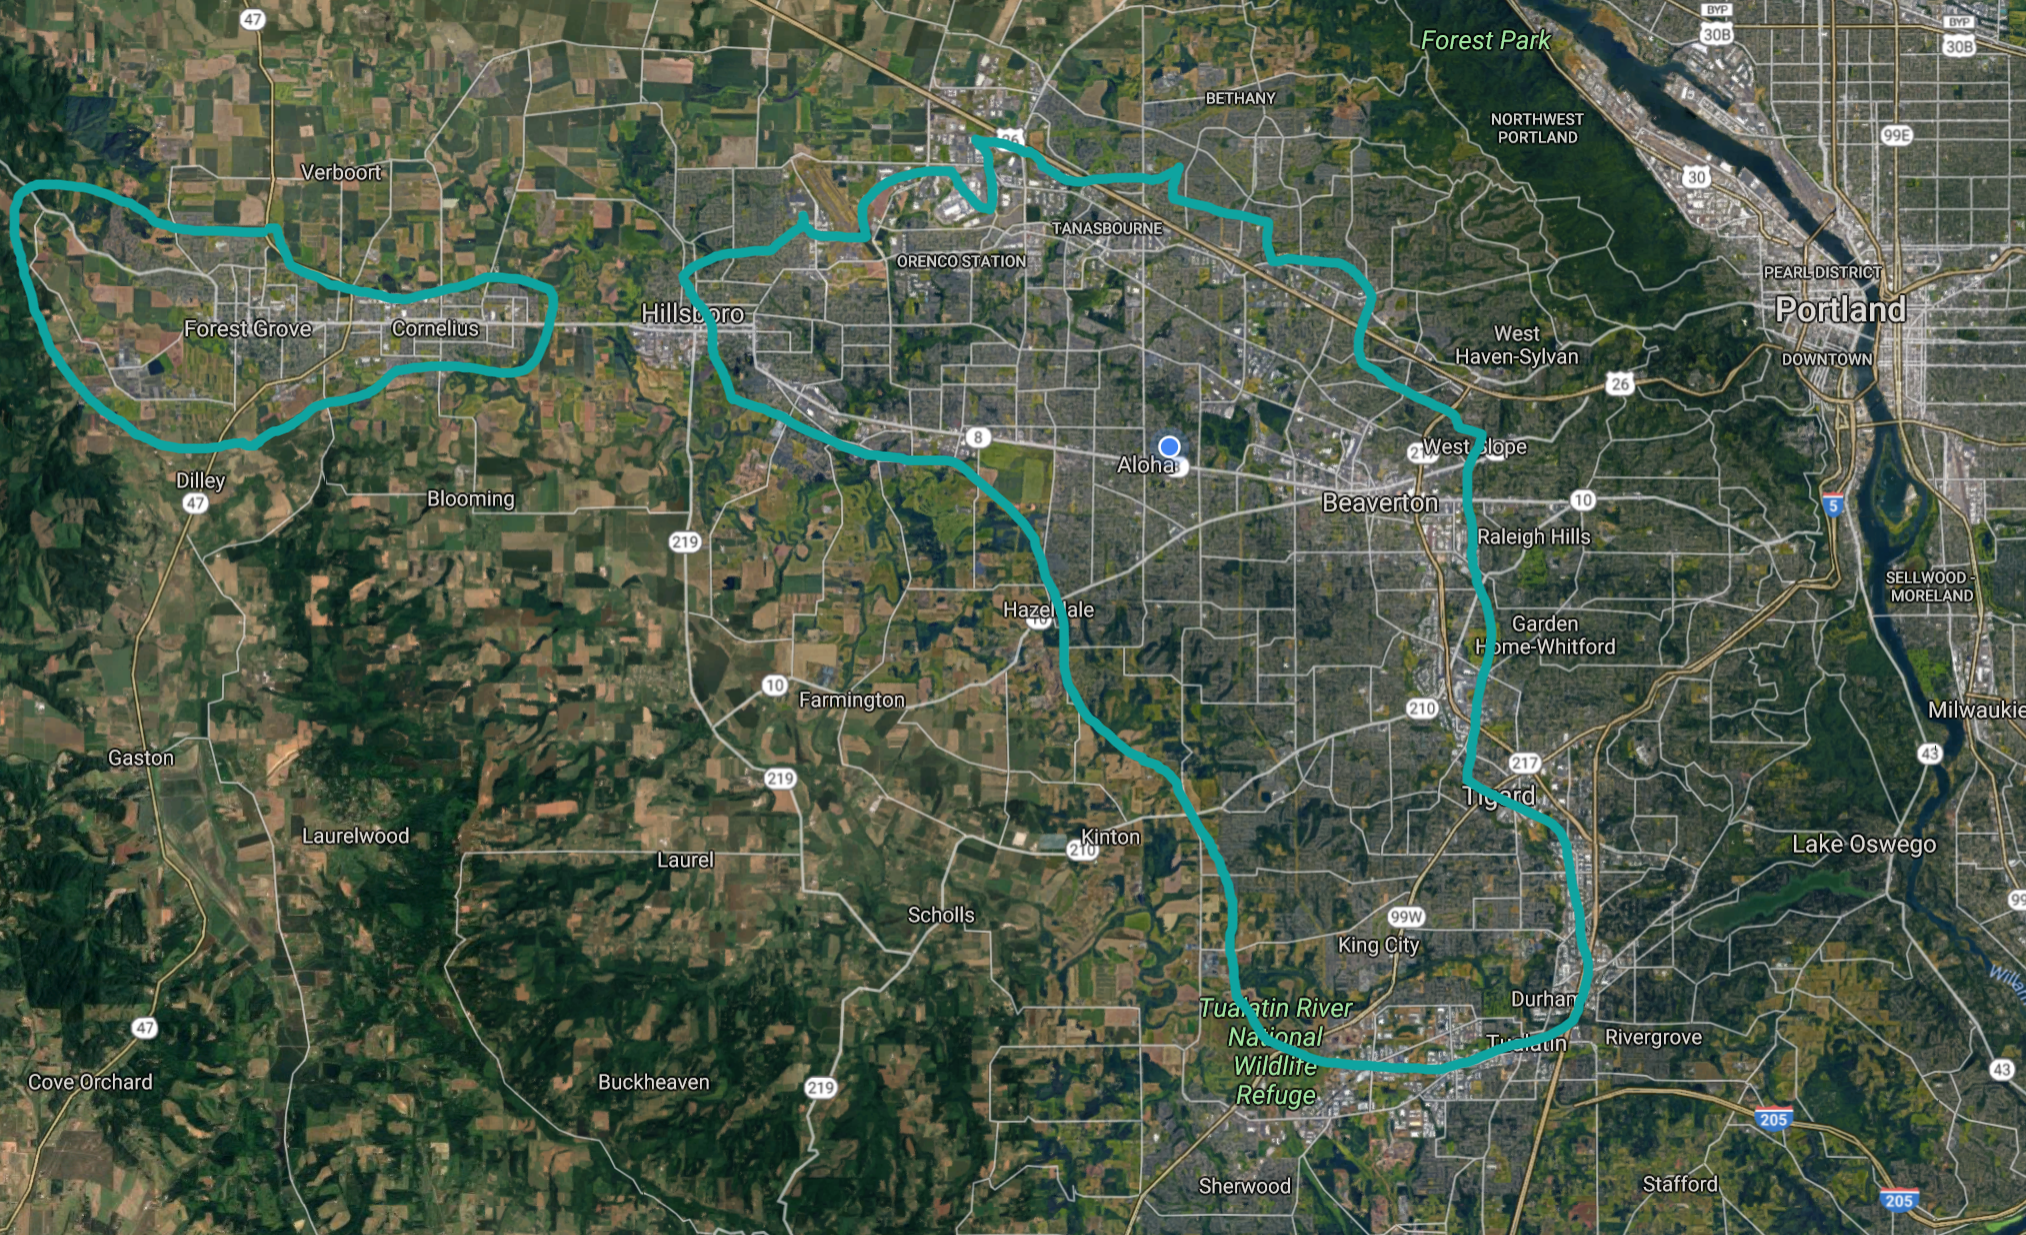
\includegraphics[width=12cm]{tualatinGMaps}
\label{gMaps}
\end{figure}

The Tualatin watershed cover approximately 1350 square miles and consists of 6 sub-watersheds. Most of these sub-watersheds
drain into the Tualatin River. Which itself is a tributary of the Willamette! 

\subsection{Features and Uses}
The Tualatin river is 83 miles long, and drains a an area called Tualatin Valley. It is considered a farming region, but
these days the area is becoming more and more populated. In fact, 20\% of the land that drains into the river
is populated with a total popluation of 500,000 people. 

As for the majority of land that composes the Tualatin Valley watershed, 30\% is agricultural, and 50\% is forest.

As can be seen in figure~\ref{tualatinValley} the Tualatin River really snakes around. Also, the figure gives a better 
idea of what is meant by the Tualatin Valley, and another feature this watershed provides, recreation! The river drains 
from the costal mountains.

\begin{figure}[H]
\centering{}
\caption{Tualatin River/Valley \href{http://tualatinriverkeepers.org/wp-content/uploads/2016/09/TRKWaterTrailBig2016.png}{\underline{--- Source}}}
\includegraphics[width=\textwidth]{tualatinRiver}\label{tualatinValley}
\end{figure}

As noted in the above figure, the Tualatin River is raised a few feet by the Scoggins dam owned by the Lake Oswego Corp.
This dam is in place to increase the water level and thus water pressure such that land downstream can use the water
for irrigation and farming purposes. 

The dam also creates what is known as Hag Lake, a local fishing and recreation spot.

The Tualatin River has five major tributaries: Scoggins Creek, Gales Creek, Dairy Creek, Rock Creek, Beaverton Creek.
The tributaries can be seen in figure~\ref{tributaries}.


\begin{figure}[H]
\centering{}
\caption{Tributaries \href{http://tualatinriverkeepers.org/wp-content/uploads/2016/09/TRKWaterTrailBig2016.png}{\underline{--- Source}}}
\includegraphics[width=\textwidth]{tualatinTributaries}\label{tributaries}
\end{figure}

It's clear that this watershed is vital to my home town. It supports both aggriculture and residency. With only 20\% 
of the watershed's land occupied by people, it isn't a watershed that needs a ton of remediation, but does still 
warrant care. The watershed's river and tributaries are monitored for common farming chemicals like fertilizers and
pesticides.

\section{Willamette Watershed}
\subsection{Overview}
Unlike the Tualatin Watershed, the Willamette Watershed doesn't even cover an entire city! Of course that's just silly 
human boundaries as it still covers nearly the same area and is vital to an even greater population. As before, figure~\ref{willOverview} shows the broad view of this watershed and its location relative to Oregon's borders.

\begin{figure}[H]
\centering{}
\caption{Willamette Watershed---Epa.gov}
\includegraphics[width=4.5cm]{willOverview}\label{willOverview}
\end{figure}

Which is again a sub-watershed of a greater system as shown in figure~\ref{willSubSheds}.

\begin{figure}[H]
\centering{}
\caption{Willamette Watershed---City of Portland}
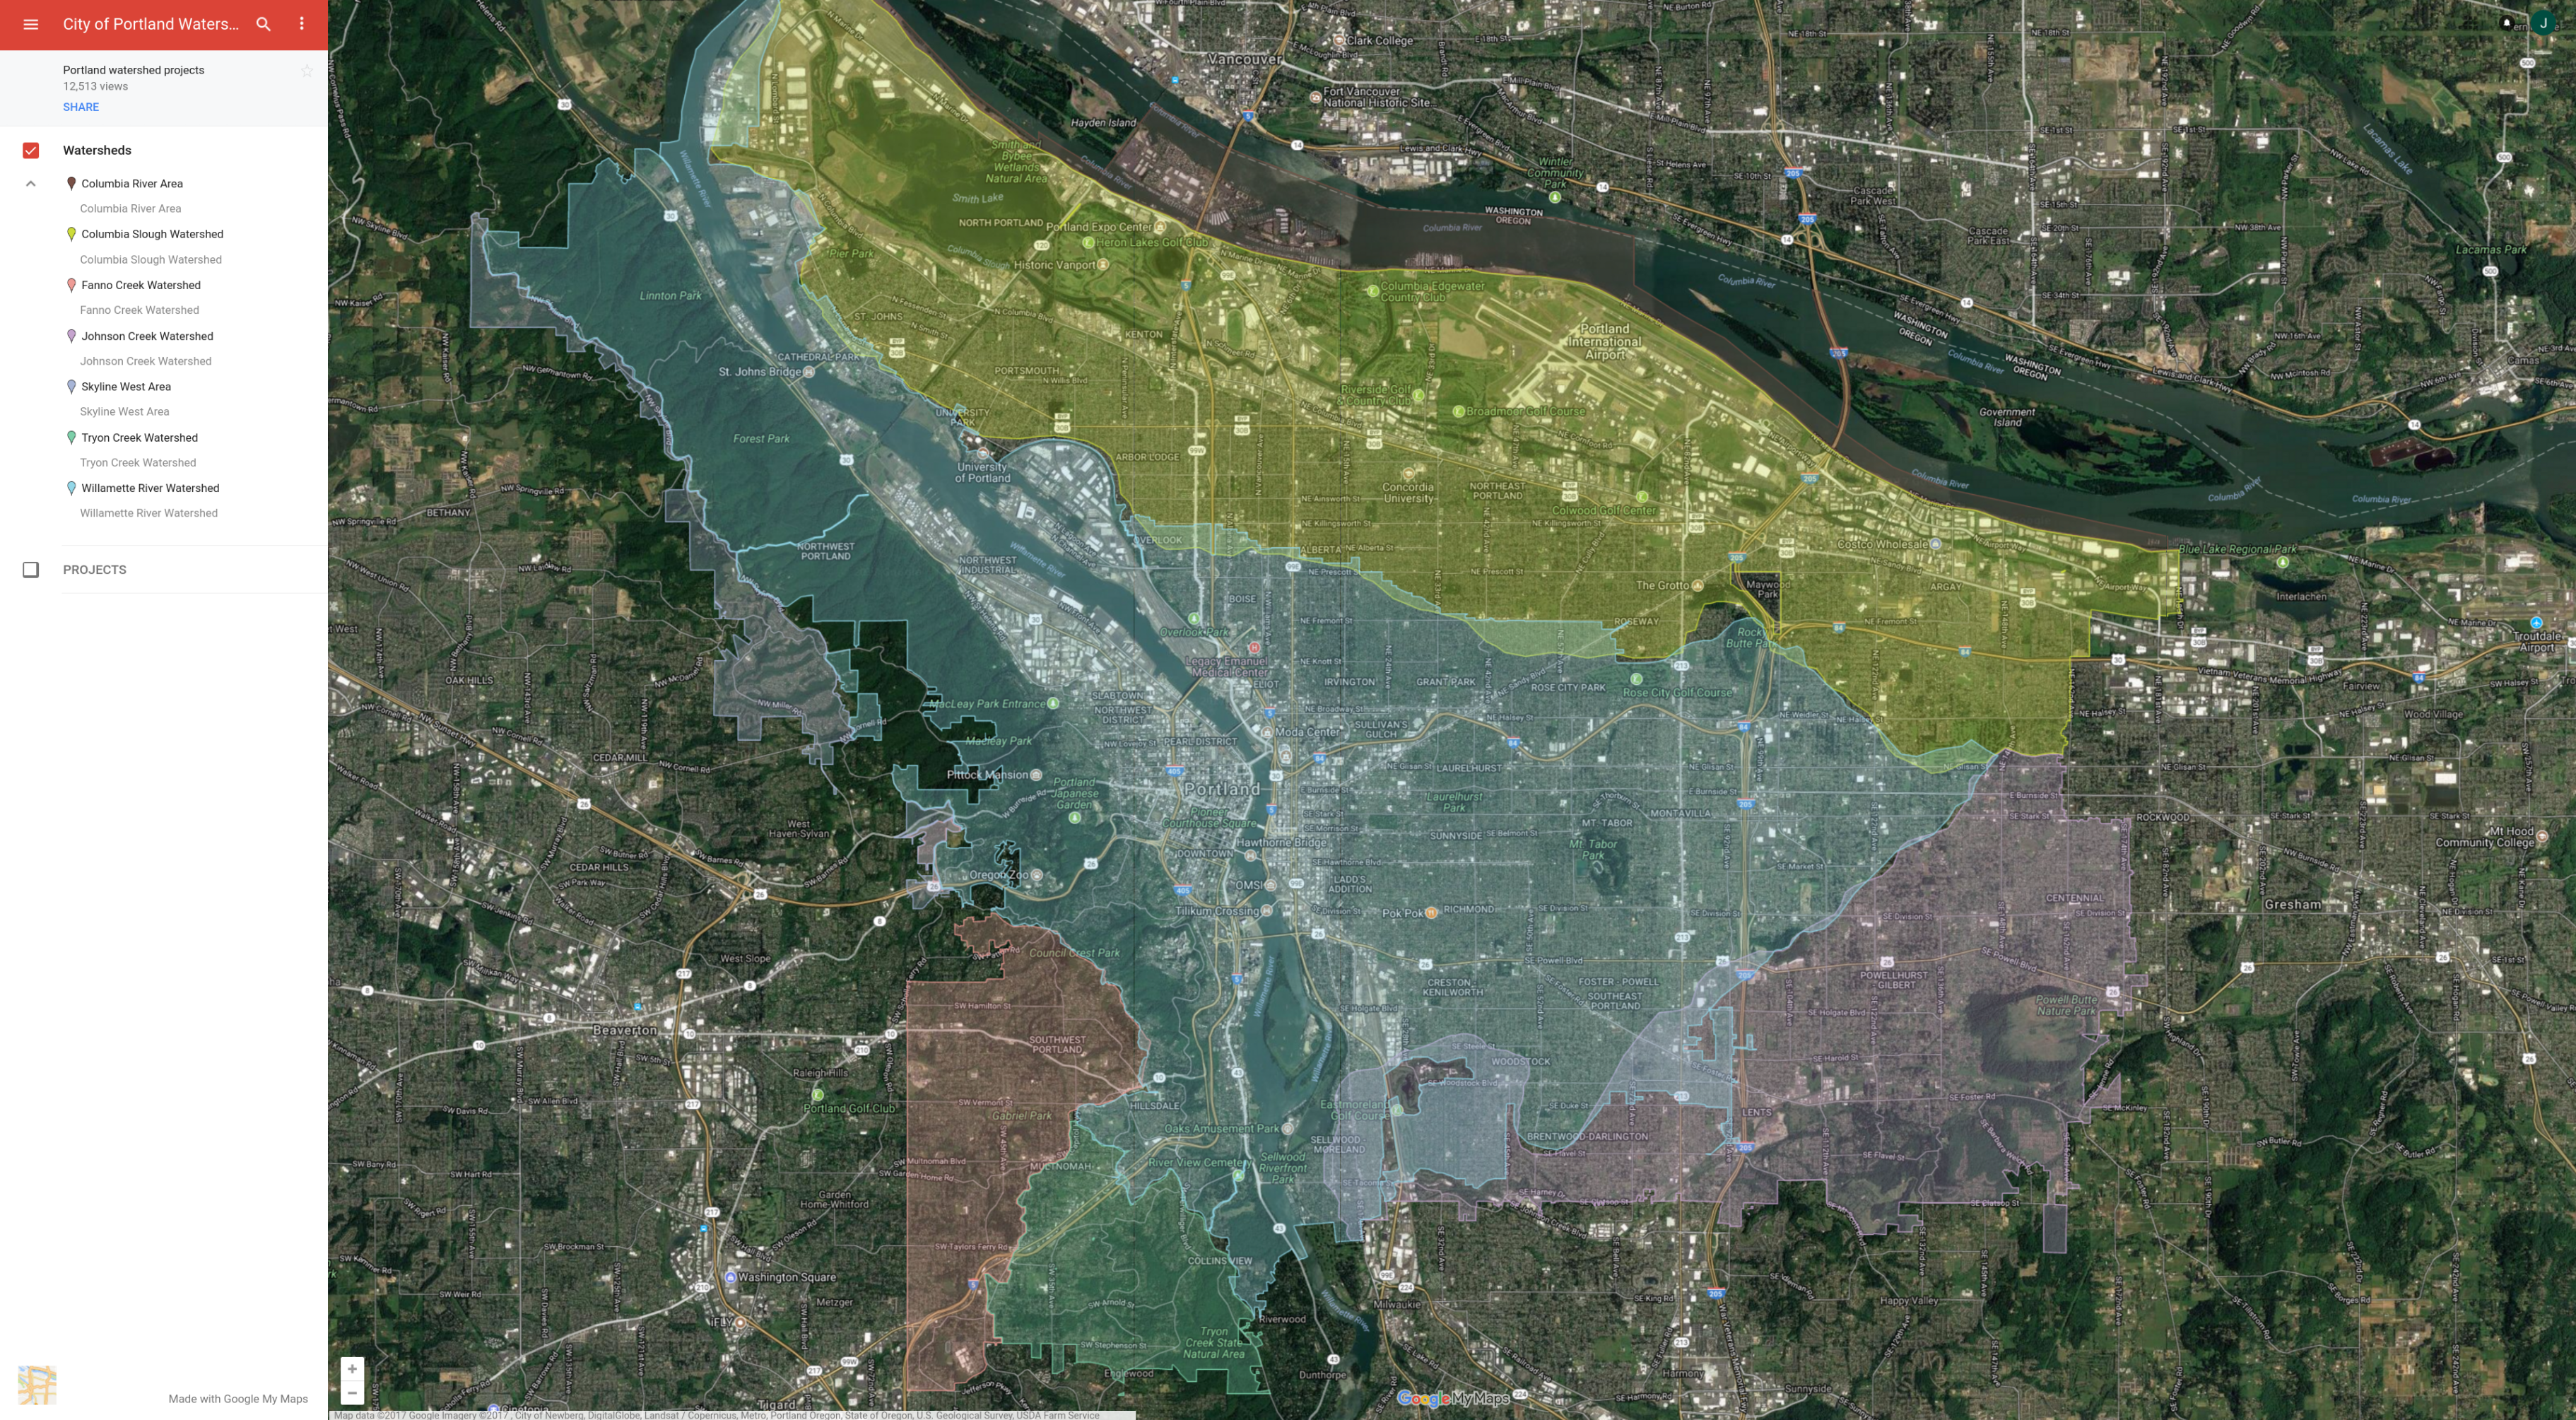
\includegraphics[width=\textwidth]{watershedsOfPortland}\label{willSubSheds}
\end{figure}


In the figure~\ref{willGMaps}, I've again drawn a border over a google map image of the water shed. In this map,
it is quite easy to see the main features of the watershed which include the Willamette River, Forest Park, and
occupied areas of Portland.

\begin{figure}[H]
\centering{}
\caption{Google Maps of Willamette Watershed}
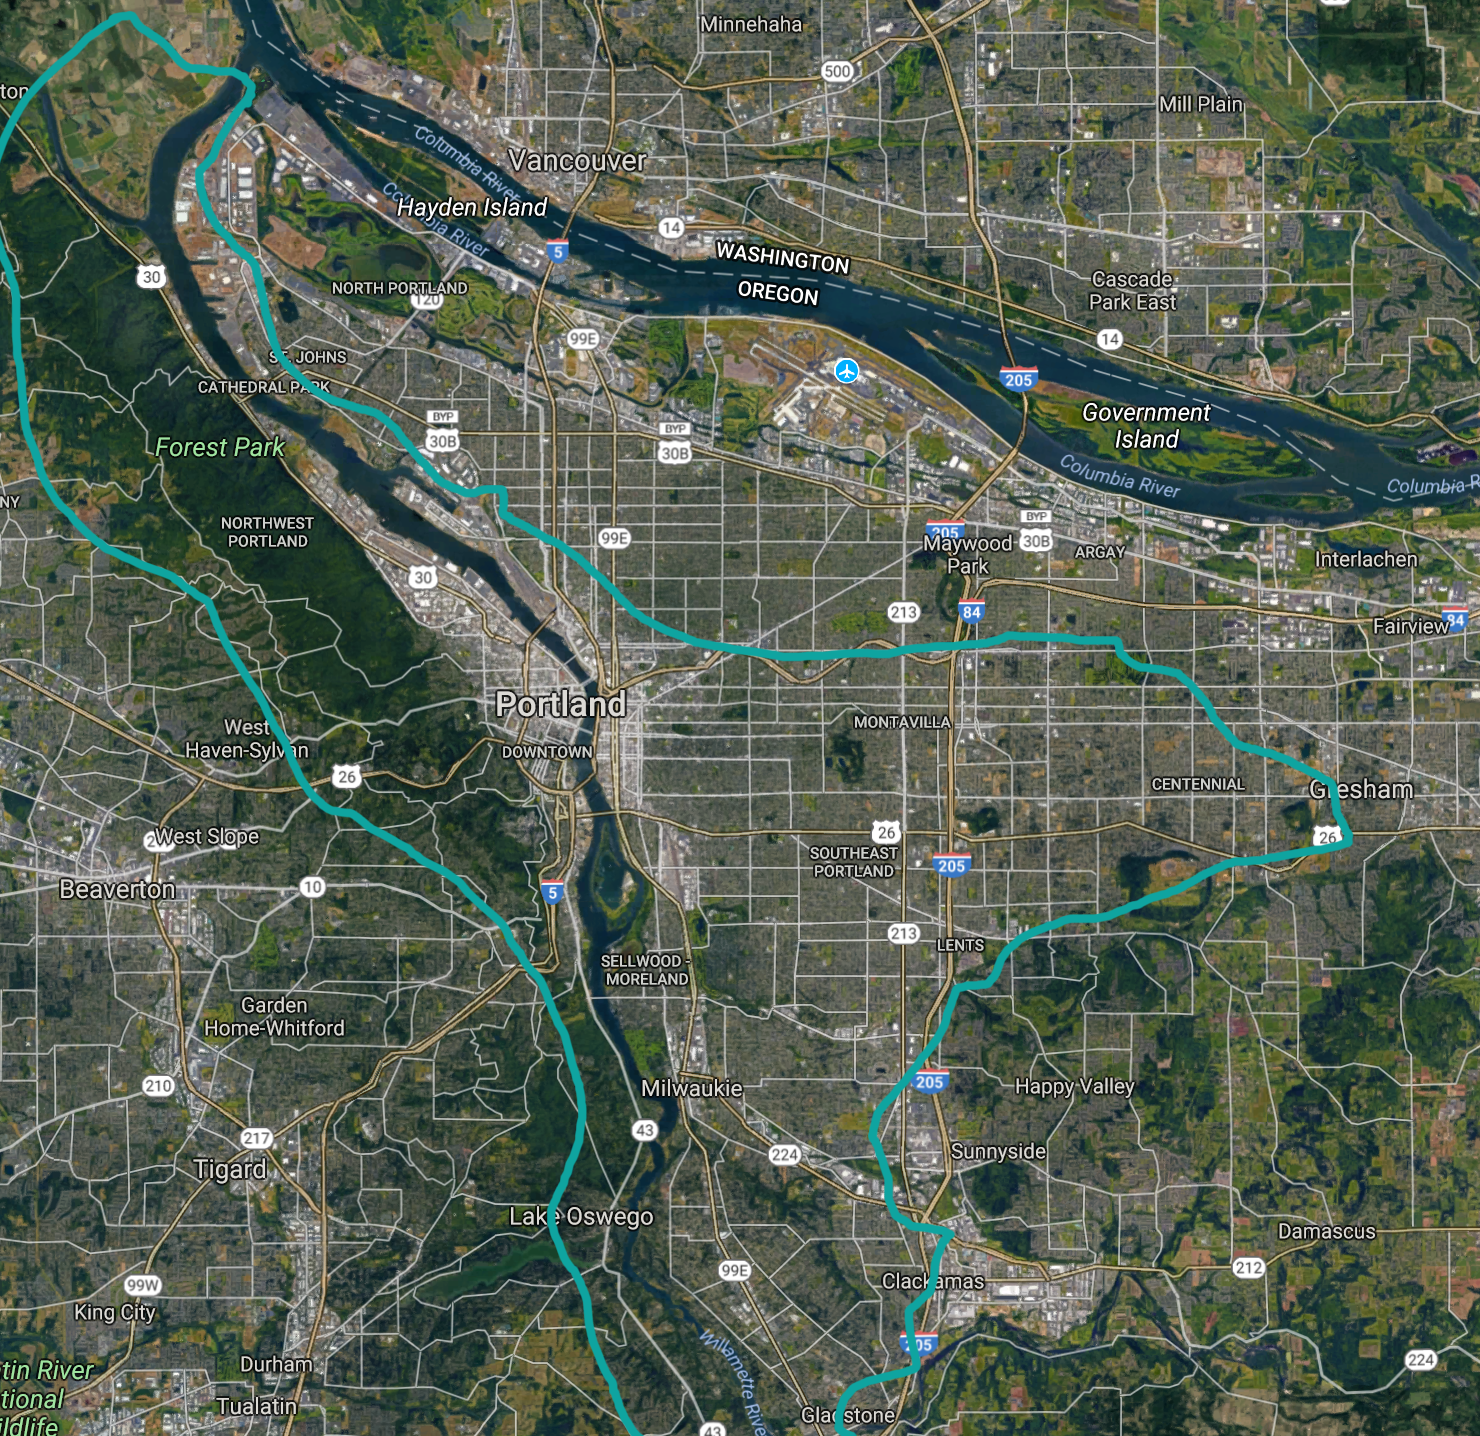
\includegraphics[width=\textwidth]{willGMaps}\label{willGMaps}
\end{figure}

\subsection{Features}
\subsubsection{Portland}
Portland is actually only a small portion of the greater watershed. About 17 miles of the Willamette runs through the city.
The Willamette actually meets with the Columbia river within Portland. The city is highly populated, yet it is still 
to the watershed as a whole. This part of the watershed is said to act as a gateway to fish and wildlife.

Urban areas require special care to prevent watershed pollution and disfunction. At any one point in time, there are usually
several watershed enhancement projects occuring. Despite the large amount of water flowing through the Willamette watershed,
the city actually uses the Bull Mountain watershed for water supply.

More below\ldots (bad formatting)

\newpage

\subsubsection{Willamette River}
The Willamette River actually originates near Euegene. This and the river's major tributaries can be seen in figure~\ref{willRiver}. The river is a source of recreation and more for the city. For example, several dams are used to generate electricity.

\begin{figure}[H]
\centering{}
\caption{Willamette River and Tributaries \href{http://trwc.org/wp-content/uploads/2013/03/Subbasins-entire.jpg}{\underline{--- Source}}}
\includegraphics[width=\textwidth]{willRiverTributaries}\label{willRiver}
\end{figure}

\subsubsection{Dams}
There are over 20 dams on the Willamette river and tributaries. There is also extensive use of levees, dikes, and channels
for flow control. The only dam on the River itself is the Willamette Falls Locks located near Oregon City as shown in 
figure~\ref{willLocks}

\begin{figure}[H]
\centering{}
\caption{Willamette Falls Locks}
\includegraphics[width=\textwidth]{willLock}\label{willLocks}
\end{figure}

\subsubsection{Forrest Park}
Forrest park is just as it sounds a large forrested park. It is over 5100 square acres, and drains into the Willamette.
It is known as a rich natural preserve with more than 112 bird species and 62 mammals. About 40 inches of rain falls on 
the park per year.

\subsubsection{Harbor}
The Willamette river is home to a harbor called the Port of Portland. This portion of the river is subject to dredging and
maintence to maintain sailability to cargo ships. Portland of course only developed as a consequence of the Columbia and 
Willamette Rivers.

Clearly the Willammette Watershed is a huge vital watershed with strongly differing maintenance needs from that of the
Tualatin watershed. The city depends on the river for cargo transport, fish depend on it for passage, and most of the
drainage comes from occupied land or forrestry as opposed to farmland.
\end{document}














